\documentclass[12pt,a4paper]{article}

\usepackage[T2A]{fontenc}
\usepackage[utf8]{inputenc}
\usepackage[russian]{babel}

\usepackage{amsmath,amssymb}
\usepackage{geometry}
\usepackage{graphicx}
\usepackage{float}
\usepackage{hyperref}
\usepackage{setspace}
\usepackage{array}
\usepackage{listings}
\usepackage{xcolor}

\geometry{margin=2cm}
\onehalfspacing

\lstdefinestyle{py}{
  language=Python,
  basicstyle=\ttfamily\small,
  keywordstyle=\color{blue!60!black},
  commentstyle=\color{green!40!black},
  stringstyle=\color{orange!50!black},
  showstringspaces=false,
  breaklines=true,
  frame=single,
  tabsize=4
}

\begin{document}

\begin{titlepage}
\begin{center}
МИНИСТЕРСТВО НАУКИ И ВЫСШЕГО ОБРАЗОВАНИЯ РФ\\
Федеральное государственное автономное\\
образовательное учреждение высшего образования\\
«Национальный исследовательский университет ИТМО»\\[0.5em]
ФАКУЛЬТЕТ ПРОГРАММНОЙ ИНЖЕНЕРИИ И КОМПЬЮТЕРНОЙ ТЕХНИКИ\\[2em]

\textbf{ЛАБОРАТОРНАЯ РАБОТА №2}\\
\textbf{по дисциплине}\\
\textbf{ВЫЧИСЛИТЕЛЬНАЯ МАТЕМАТИКА}\\[0.5em]
Вариант №3\\[2em]
\end{center}

\vfill

\begin{flushright}
\begin{tabular}{@{}l@{}}
Выполнил:  Григорьев Даниил Александрович\\
студент группы P3216\\
\\
\\
Преподаватель:  Наумова Надежда Александровна\\
\end{tabular}
\end{flushright}

\vfill

\begin{center}
Санкт-Петербург, 2026
\end{center}
\end{titlepage}

\section*{Цель работы}
Изучить численные методы решения нелинейных уравнений и их систем, найти корни заданного нелинейного уравнения и заданной системы, выполнить программную реализацию методов.

\section*{Анализ задания}
По таблицам 6--9 задания для варианта 3:
\begin{enumerate}
\item Нелинейное уравнение:
\[
x^3+2.84x^2-5.606x-14.766=0.
\]
\item Методы для вычислительной части 1 (таблица 7):
\begin{itemize}
\item крайний левый корень --- метод простой итерации (код 5),
\item центральный корень --- метод Ньютона (код 3),
\item крайний правый корень --- метод половинного деления (код 1).
\end{itemize}
\item Система (таблица 8):
\[
\begin{cases}
\cos(x-1)+y=0.5,\\
x-\cos y=3,
\end{cases}
\]
метод --- простая итерация.
\item Методы, требуемые в программной реализации (таблица 9):
\begin{itemize}
\item для уравнений: 2, 4, 5,
\item для систем: 6.
\end{itemize}
В программе реализованы эти методы, а также дополнительные методы для полноты.
\end{enumerate}

\section*{Ход работы, расчетные формулы}

\subsection*{Часть 1. Нелинейное уравнение}
Рассматриваем:
\[
f(x)=x^3+2.84x^2-5.606x-14.766.
\]

\subsubsection*{1.1. Отделение корней}
Проверка знаков функции:
\begin{figure}
    \centering
    \includegraphics[width=0.5\linewidth]{figures/graphic1.png}
    \caption{График f(x)}
    \label{fig:placeholder}
\end{figure}
\[
f(-4)=-10.902<0,\quad f(-3)=0.612>0 \Rightarrow x_1\in(-4,-3),
\]
\[
f(-3)=0.612>0,\quad f(-2)=-0.194<0 \Rightarrow x_2\in(-3,-2),
\]
\[
f(2)=-6.618<0,\quad f(3)=20.976>0 \Rightarrow x_3\in(2,3).
\]

\subsubsection*{1.2. Левый корень методом простой итерации}
Берем преобразование
\[
x=\varphi(x)=x-\lambda f(x),\qquad
\]

Подберем \(\lambda\) из условия сходимости метода простой итерации:
\[
|\varphi'(x)|<1 \quad \text{на выбранном интервале}.
\]

Имеем
\[
\varphi'(x)=1-\lambda f'(x),
\]
где
\[
f'(x)=3x^2+5.68x-5.606.
\]

Для левого корня рассматриваем интервал \([-4;\,-3]\). Чтобы проверка была
выполнена не только на границах, а на всём интервале, исследуем поведение
производной \(f'(x)\). Имеем
\[
f''(x)=6x+5.68.
\]
На интервале \([-4;\,-3]\)
\[
f''(-4)=-18.32<0,\qquad f''(-3)=-12.32<0,
\]
следовательно, \(f''(x)<0\) для всех \(x\in[-4,-3]\), а значит функция
\(f'(x)\) убывает на всём рассматриваемом интервале.

Тогда максимум и минимум \(f'(x)\) на интервале достигаются на его концах:
\[
\max_{x\in[-4,-3]} f'(x)=f'(-4)=3\cdot 16+5.68\cdot(-4)-5.606=19.674,
\]
\[
\min_{x\in[-4,-3]} f'(x)=f'(-3)=3\cdot 9+5.68\cdot(-3)-5.606=4.354.
\]

Следовательно, для любого \(x\in[-4,-3]\) выполняется оценка
\[
4.354\le f'(x)\le 19.674.
\]

Выберем \(\lambda=0.08\). Тогда для любого \(x\in[-4,-3]\)
\[
\varphi'(x)=1-0.08\,f'(x).
\]
Так как \(f'(x)\in[4.354;\,19.674]\), получаем
\[
1-0.08\cdot 19.674 \le \varphi'(x) \le 1-0.08\cdot 4.354,
\]
\[
-0.574 \le \varphi'(x) \le 0.652.
\]

Следовательно,
\[
q=\max_{x\in[-4,-3]}|\varphi'(x)|
\le \max(0.574,\;0.652)=0.652<1.
\]



Условие сходимости выполнено.

Начальное приближение: $x_0=-4$, $\varepsilon=0.01$.

\begin{table}[H]
\centering
\caption{Метод простой итерации (левый корень)}
\begin{tabular}{|c|c|c|c|c|}
\hline
№ итерации & $x_k$ & $x_{k+1}$ & $f(x_{k+1})$ & $|x_{k+1}-x_k|$ \\
\hline
1 & -4.000 & -3.128 & -0.047 & 0.872 \\
\hline
2 & -3.128 & -3.124 & -0.025 & 0.004 \\
\hline
\end{tabular}
\end{table}

Итак,
\[
x_1\approx -3.124.
\]

\subsubsection*{1.3. Центральный корень методом Ньютона}
Используем формулу:
\[
x_{k+1}=x_k-\frac{f(x_k)}{f'(x_k)}.
\]
Начальное приближение: $x_0=-2$, $\varepsilon=0.01$.

\begin{table}[H]
\centering
\caption{Метод Ньютона (центральный корень)}
\begin{tabular}{|c|c|c|c|c|c|}
\hline
№ итерации & $x_k$ & $f(x_k)$ & $f'(x_k)$ & $x_{k+1}$ & $|x_{k+1}-x_k|$ \\
\hline
1 & -2.000 & -0.194 & -4.966 & -2.039 & 0.039 \\
\hline
2 & -2.039 & -0.005 & -4.715 & -2.040 & 0.001 \\
\hline
\end{tabular}
\end{table}

Следовательно,
\[
x_2\approx -2.040.
\]

\subsubsection*{1.4. Правый корень методом половинного деления}
Используем интервал изоляции $[2,3]$.

Формулы метода:
\[
x_k=\frac{a_k+b_k}{2},
\]
если $f(a_k)f(x_k)\le0$, то $b_{k+1}=x_k$, иначе $a_{k+1}=x_k$.

\begin{table}[H]
\centering
\caption{Метод половинного деления (правый корень)}
\begin{tabular}{|c|c|c|c|c|c|c|c|}
\hline
№ шага & $a$ & $b$ & $x$ & $f(a)$ & $f(b)$ & $f(x)$ & $|b-a|$ \\
\hline
1 & 2.000 & 3.000 & 2.500 & -6.618 & 20.976 & 4.594 & 1.000 \\
\hline
2 & 2.000 & 2.500 & 2.250 & -6.618 & 4.594 & -1.611 & 0.500 \\
\hline
3 & 2.250 & 2.500 & 2.375 & -1.611 & 4.594 & 1.336 & 0.250 \\
\hline
4 & 2.250 & 2.375 & 2.313 & -1.611 & 1.336 & -0.176 & 0.125 \\
\hline
5 & 2.313 & 2.375 & 2.344 & -0.176 & 1.336 & 0.570 & 0.063 \\
\hline
6 & 2.313 & 2.344 & 2.328 & -0.176 & 0.570 & 0.195 & 0.031 \\
\hline
7 & 2.313 & 2.328 & 2.320 & -0.176 & 0.195 & 0.009 & 0.016 \\
\hline
\end{tabular}
\end{table}

Так как $|f(x_7)|=0.009<0.01$, получаем:
\[
x_3\approx 2.320.
\]

\subsubsection*{1.5. Ответ по уравнению}
Итоговые корни:
\[
x_1\approx -3.124,\qquad x_2\approx -2.040,\qquad x_3\approx 2.320.
\]


\subsection*{Часть 2. Система нелинейных уравнений}
Система варианта 3:
\[
\begin{cases}
\cos(x-1)+y=0.5,\\
x-\cos y=3.
\end{cases}
\]
\begin{figure}[H]
    \centering
    \includegraphics[width=0.5\linewidth]{figures/graphic2.png}
    \caption{ГРафик системы}
    \label{fig:placeholder}
\end{figure}

Метод: простая итерация.
Переходим к виду
\[
\begin{cases}
x=\varphi_1(x,y)=3+\cos y,\\
y=\varphi_2(x,y)=0.5-\cos(x-1).
\end{cases}
\]

\subsubsection*{2.1. Проверка сходимости}
Частные производные:
\[
\frac{\partial\varphi_1}{\partial x}=0,\quad
\frac{\partial\varphi_1}{\partial y}=-\sin y,
\]
\[
\frac{\partial\varphi_2}{\partial x}=\sin(x-1),\quad
\frac{\partial\varphi_2}{\partial y}=0.
\]

В области локализации решения
\[
3.30\le x\le 3.40,\qquad 1.20\le y\le 1.22
\]
получаем:
\[
\left|\frac{\partial\varphi_1}{\partial x}\right|+
\left|\frac{\partial\varphi_1}{\partial y}\right|
\le \sin(1.22)\approx 0.939,
\]
\[
\left|\frac{\partial\varphi_2}{\partial x}\right|+
\left|\frac{\partial\varphi_2}{\partial y}\right|
\le \sin(2.4)\approx 0.746.
\]

Следовательно,
\[
q=\max(0.939,\,0.746)=0.939<1,
\]
достаточное условие сходимости выполнено.

\subsubsection*{2.2. Итерационный процесс}
Берем начальное приближение
\[
x^{(0)}=3.35,\qquad y^{(0)}=1.20,
\]
критерий остановки
\[
\max\left(|x^{(k+1)}-x^{(k)}|,\,|y^{(k+1)}-y^{(k)}|\right)<0.01.
\]

\begin{table}[H]
\centering
\caption{Метод простой итерации для системы}
\begin{tabular}{|c|c|c|c|c|c|c|}
\hline
№ итерации & $x^{(k)}$ & $y^{(k)}$ & $x^{(k+1)}$ & $y^{(k+1)}$ & $|\Delta x|$ & $|\Delta y|$ \\
\hline
1 & 3.350 & 1.200 & 3.362 & 1.203 & 0.012 & 0.003 \\
\hline
2 & 3.362 & 1.203 & 3.360 & 1.211 & 0.003 & 0.009 \\
\hline
\end{tabular}
\end{table}

На второй итерации условие остановки выполнено. Получаем:
\[
x\approx 3.360,\qquad y\approx 1.211.
\]

Проверка подстановкой:
\[
\cos(x-1)+y-0.5\approx 1.78\cdot 10^{-3},
\]
\[
x-\cos y-3\approx 8.17\cdot 10^{-3}.
\]

\begin{center}
\IfFileExists{figures/system_variant3.png}{
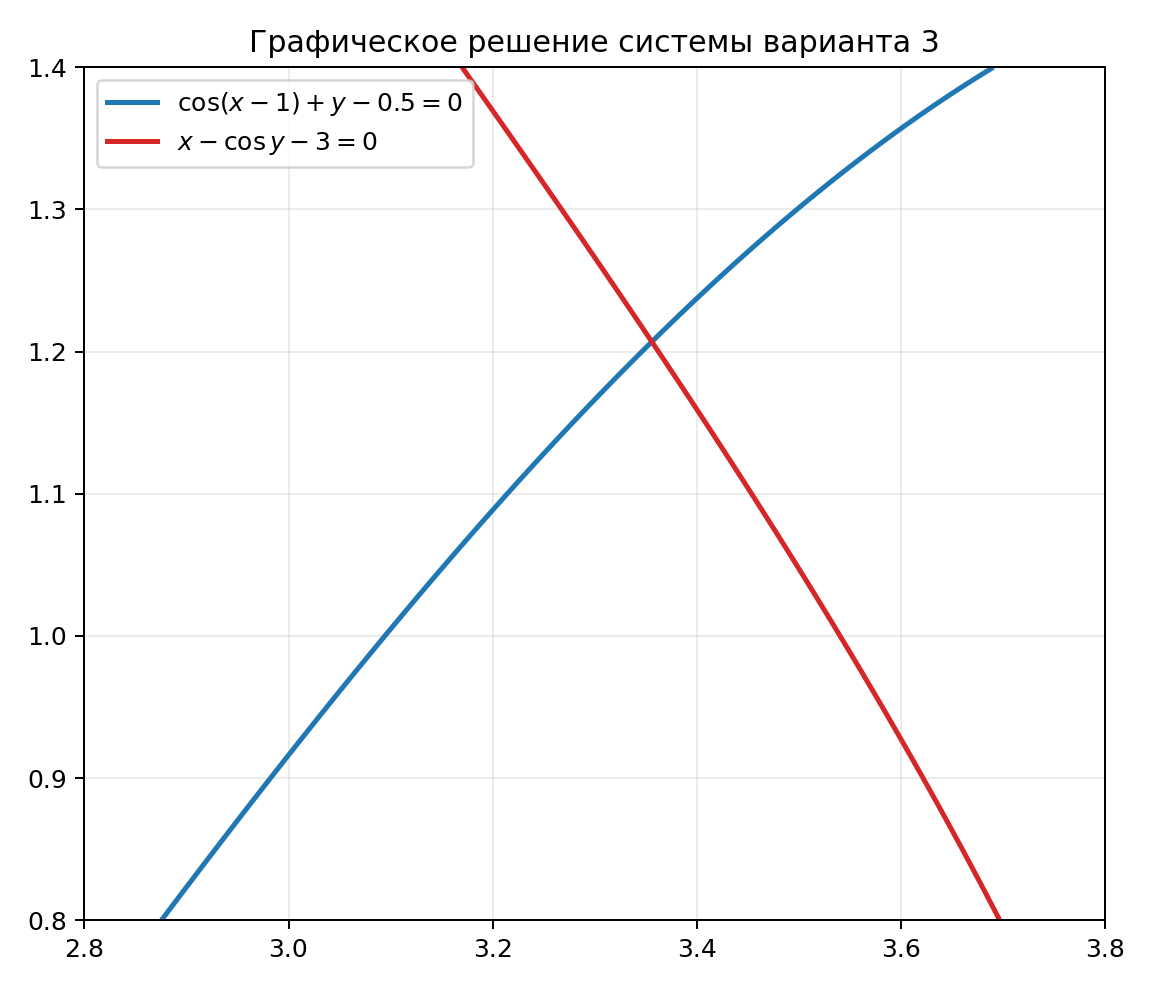
\includegraphics[width=0.85\textwidth]{figures/system_variant3.png}
}{
\fbox{\parbox{0.85\textwidth}{\centering}}}
\end{center}

\subsubsection*{2.3. Ответ по системе}
Итак, с точностью \(\varepsilon=0.01\) решение системы имеет вид
\[
x\approx 3.360,\qquad y\approx 1.211.
\]

\section*{Блок-схемы}
\begin{figure}[H]
    \centering
    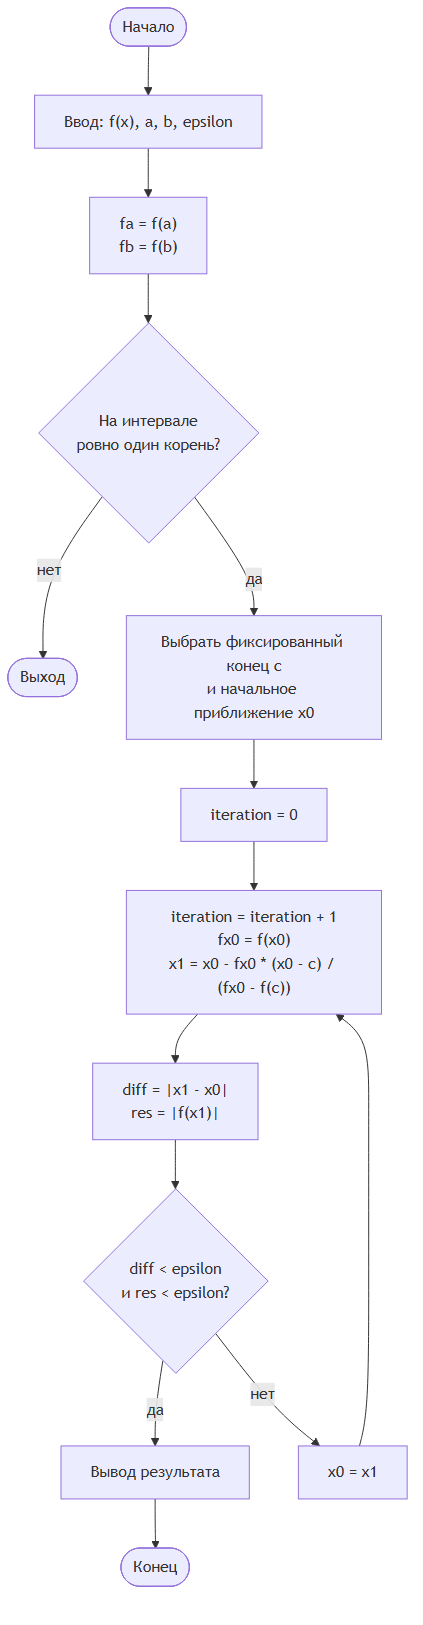
\includegraphics[width=0.78\textwidth]{program_part/diagrams/chord_method.png}
    \caption{Блок-схема метода хорд}
\end{figure}

\begin{figure}[H]
    \centering
    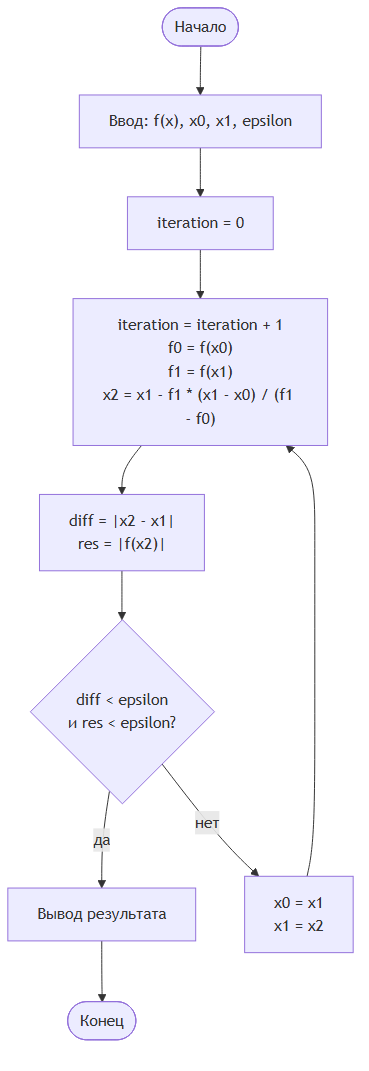
\includegraphics[width=0.78\textwidth]{program_part/diagrams/secant_method.png}
    \caption{Блок-схема метода секущих}
\end{figure}

\begin{figure}[H]
    \centering
    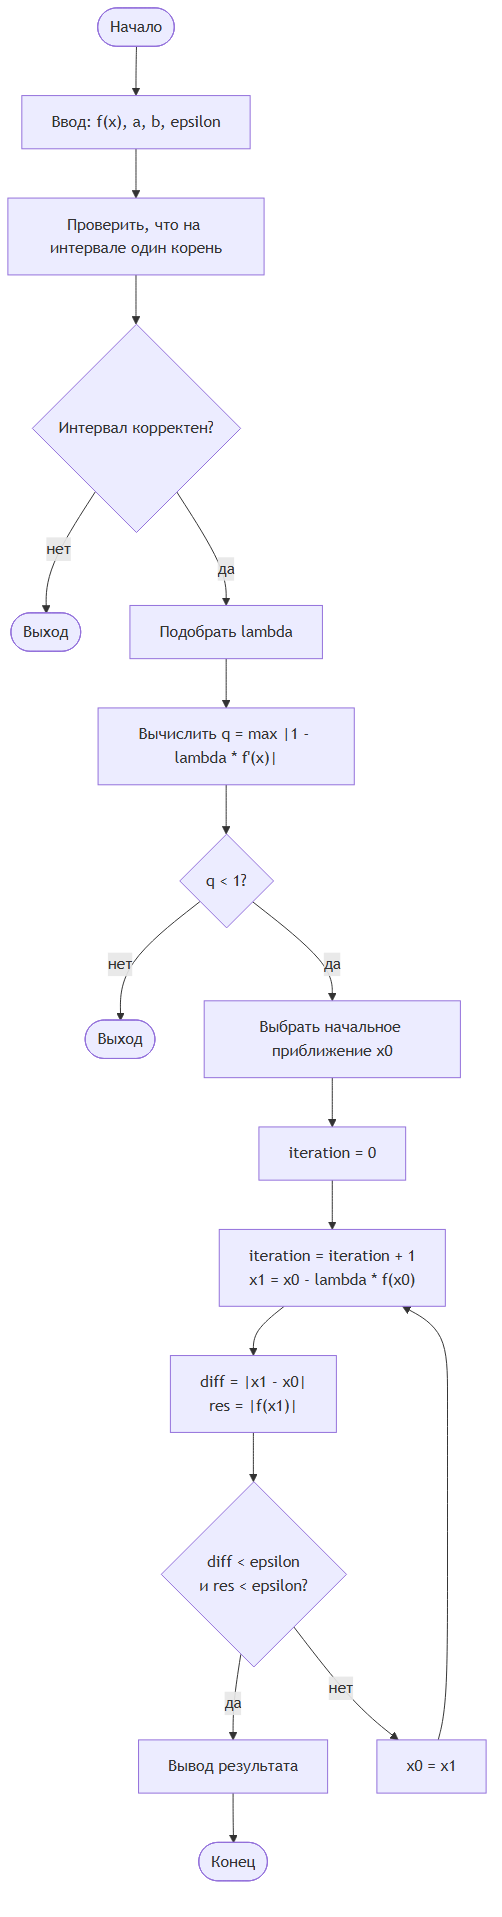
\includegraphics[width=0.78\textwidth]{program_part/diagrams/simple_iteration_method.png}
    \caption{Блок-схема метода простой итерации}
\end{figure}

\begin{figure}[H]
    \centering
    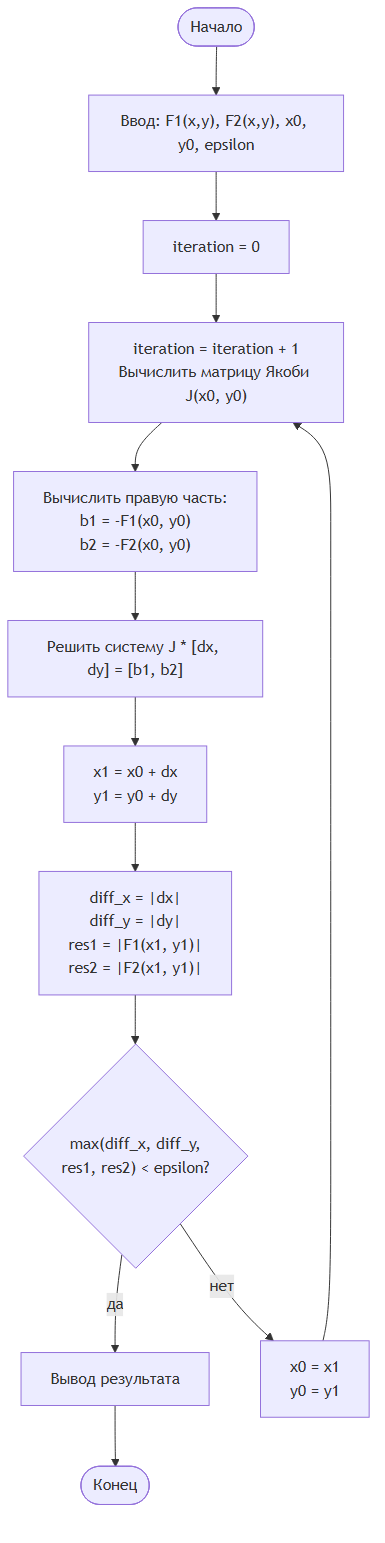
\includegraphics[width=0.78\textwidth]{program_part/diagrams/newton_system_method.png}
    \caption{Блок-схема метода Ньютона для системы нелинейных уравнений}
\end{figure}

\section*{Программная реализация}
Программная часть лабораторной работы реализована на языке Python в виде
настольного приложения с графическим интерфейсом пользователя. В качестве
точки входа используется файл \texttt{main.py}, который запускает модуль
\texttt{program\_part/main.py}. Интерфейс приложения построен с помощью
\texttt{tkinter}, а графики функций и систем отображаются с использованием
\texttt{matplotlib}.

Программа поддерживает методы, требуемые заданием для программной реализации:
\begin{itemize}
\item для нелинейных уравнений: метод хорд, метод секущих, метод простой итерации;
\item для систем нелинейных уравнений: метод Ньютона.
\end{itemize}

Структура программной части:
\begin{itemize}
\item \texttt{main.py} --- внешний файл запуска приложения;
\item \texttt{program\_part/main.py} --- запуск графического интерфейса;
\item \texttt{program\_part/gui\_app.py} --- окно приложения, элементы управления, обработчики кнопок, область графика и текстовый вывод результатов;
\item \texttt{program\_part/solver\_service.py} --- сервисный слой, объединяющий проверку входных данных и запуск нужного численного метода;
\item \texttt{program\_part/equation\_methods.py} --- реализация методов хорд, секущих и простой итерации для уравнений;
\item \texttt{program\_part/system\_methods.py} --- реализация метода Ньютона для систем;
\item \texttt{program\_part/equation\_problems.py} и \texttt{program\_part/system\_problems.py} --- наборы уравнений и систем;
\item \texttt{program\_part/io\_utils.py} --- формирование текстовых отчетов по результатам вычислений;
\item \texttt{program\_part/number\_utils.py} --- разбор вещественных чисел, в том числе с десятичной запятой, и форматирование вывода;
\item \texttt{program\_part/plotting\_utils.py} --- построение графиков уравнений и систем.
\end{itemize}

Программа позволяет:
\begin{enumerate}
\item выбрать один из методов \(2, 4, 5, 6\);
\item выбрать уравнение или систему из предложенного набора;
\item вводить исходные данные через графический интерфейс;
\item корректно обрабатывать вещественные числа как с точкой, так и с запятой;
\item проверять корректность интервала и наличие на нём единственного корня для методов решения уравнений;
\item автоматически выбирать фиксированный конец, начальные приближения и параметр \(\lambda\), если это требуется методом;
\item выводить таблицу итераций, найденное решение и значения невязок в текстовой области окна;
\item строить график выбранной функции или системы и отображать найденный корень (или решение системы) непосредственно на графике;
\item выводить человекочитаемые сообщения об ошибках при некорректном вводе данных.
\end{enumerate}

Ниже приведён фрагмент программы, реализующий графический интерфейс и основной
сценарий взаимодействия пользователя с численными методами.

\lstinputlisting[style=py]{program_part/gui_app.py}

\section*{Ссылка на репозиторий}
\url{https://github.com/your-username/your-repo}

\section*{Вывод}
Лабораторная работа полностью выполнена для варианта 3: решено заданное нелинейное уравнение и заданная система уравнений с точностью $\varepsilon=0.01$, проведена проверка условий сходимости для методов простой итерации и подготовлена программная реализация требуемых численных методов на Python.

\end{document}
